% !TeX root = proposal.tex

\chapter{Exploring the Acceptability of IoT (original work)}\label{chapter:acceptability}

Given the benefits and drawbacks of IoT, it becomes necessary to investigate the factors that affect users’ decision when they consider adopting the IoT technology from users' perspective. Knowing these factors is helpful and supportive to our following research because: 1) The factors that affect users' adopting phase may have a high chance to also have effect on users' real using phase; 2) These factors may help us understand how general IoT users make privacy decisions when they share their personal data in different IoT contexts; 3) These factors may further affect how we design the user interface for setting privacy preferences and recommend privacy-settings for different IoT contexts; 4) These factors may affect how we model the evaluation to the final interfaces that we design.

This chapter presents a preliminary/pilot study which was conducted on Clemson University Campus with an aim to investigate the various aspects involved in accepting technologies by the potential IoT users (On campus students primarily). By conducting this pilot study, we try to gain deeper understanding on the general IoT acceptability from users' perspective, i.e. \textbf{What are the factors that affect users' decision when they consider adopting a new IoT device}. The reason we conduct this preliminary user study is that IoT device users in real usage context would more likely pay higher attention to those factors that have already affected their decisions when they are considering adopting a IoT device, i.e. The factors that affect users' adopting phase would more likely to have effect on their real use phase too. Therefore, knowing what aspects of IoT are important to user when they are considering adopting IoT would be helpful and supportive to our following investigation on how general IoT users make decisions when they share their personal data in different IoT contexts and further affect how we design the user interface for setting privacy preferences and recommend privacy settings for different IoT contexts. I first discuss the experimental setup of our preliminary user study. Secondly, I demonstrate the analysis on the results of the study, and finally summarize our findings.

\section{Methods}
The interviews were approximately 30-50 minutes in length and covered a wide range of open questions related to IoT. These questions need participants to input their personal preferences about technology and self-perceived tech savviness. In this interview study, the conversations with our participants were recorded only after obtaining their consent. This study was approved by IRB. The entire recorded conversation was then transcribed manually. We then extracted keywords from participants' statements during the interview, such as ``privacy'' or ``ease of use''. These keywords were then grouped using card sorting and affinity diagram techniques. And finally we analyze the results.

% \begin {table}
% \caption {Participants Demographics} \label{tab:demographics1}
% \begin{center}
% 	\begin{tabular}{c|c|c}
% 		\hline
% 		Age Range & \multicolumn{2}{c}{ 21-35 }\\
% 		\hline
% 		& Male & 8 \\
% 		\cline{2-3}
% 		Gender    & Female & 2 \\
% 		\hline
% 		& Chinese & 2 \\
% 		\cline{2-3}
% 		Races 	  & Indians & 4 \\
% 		\cline{2-3}
% 		& Americans & 3 \\
% 		\cline{2-3}
% 		& Latin American & 1\\
% 		\hline
% 	\end{tabular}
% \end{center}
% \end {table}


\section{Results}
From our study, the factors that affect the acceptance of IoT devices can be summarized into following three aspects: Privacy, Usability, and Affordability. As shown in Figure~\ref{fig:AcceptingProcess}, while making the decision on whether to adopt the IoT technology, the users do a three-way calculus based on the trade-off between privacy, usability and affordability. Users are more likely to adopt an IoT device with high usability, privacy, and affordability. Within the above three aspects, only the usability and privacy  are relevant to our research questions. Although we can not do anything to affordability aspect in our study, the results still provide a good insight for manufacturers about the trade-off between usability, privacy, and affordability. Next, we present our analysis to the effect of usability and privacy to the acceptability of IoT systems/devices.

\begin{figure}[htb]
	\centering
	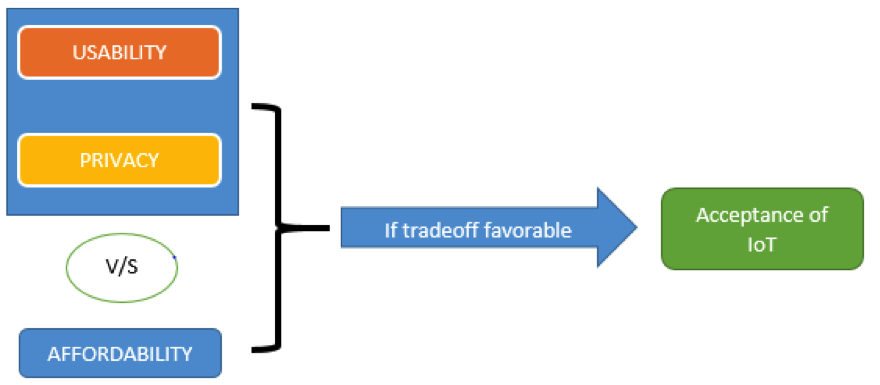
\includegraphics[width=0.6\columnwidth]{figures/AcceptingProcess.png}
	\caption{Process of accepting IoT as observed}
	\label{fig:AcceptingProcess}
\end{figure}

\subsection{IoT Privacy and Acceptability}
In this section, we present the relation between privacy concerns and the acceptability of IoT systems. The most noticeable characteristic of a IoT system is that there exists a constant sharing of information during the usage of such systems. For example, in an environment of Household IoT, a refrigerator can sense what items are stored inside it and can notify users when they need to refill the groceries. The entire IoT systems are highly relying on such data collections and sharing in order to provide the best possible experience for the users. However, users may find some of these data collections to be intrusive in nature. The perceived risks from the data collection and sharing can be the main obstacle that prevents users from adopting an IoT system. As one of the participants mentioned, 

``As long as the privacy issue can be managed and the companies can be responsible in keeping encrypted data so that it can't be easily hacked and all that. As long as everybody is respecting that privacy. I love it." 

Therefore, we consider privacy as one of the most important key factors affect users when they are making decision on whether to adopt an IoT system.

\subsubsection{Type of Information: \textit{What is collected/shared}}
Various types of information can be collected/shared in an IoT system, such as location, photos, voice, and videos. From our interviews, we observed that participants showed different levels of privacy concerns on different types of information about them being collected or shared. 

For example,
%some user will show high privacy concern about his/her photos or videos being shared, but not mind sharing his/her location. B
below is an excerpt from an interview which highlights the importance of what information is collected/shared:\\

\textit{I: ``So you are not ok with photo, video or voice?''\\}

\textit{P: ``Yes that's s pretty good generalization. Any data that is visuals of me photographs, voice, video, I would probably not want to store it.''\\}

\textit{I: ``About voice?''\\}

\textit{P: ``I mean, I understand that it is being stored to improve your algorithms but what if that was to get leaked.''\\}

Within the various types of personal information that can be collected or shared, some information can be used to help identify users' identity or even hack or rob the users, such as photos and videos. We define this type of personal information as \textbf{\textit{Identifiable Information}}.

Typically, users are mostly not comfortable with sharing their \textit{identifiable information} in an IoT system. They worried about sharing this type of data as it could threaten their security. However, some participants seem to have different sharing intention on certain types of \textit{identifiable information}. Some participant expressed that he/she doesn't mind his/her location information being shared, \textit{``At this point I am not much concerned about my location being shared. I mean if somebody wants to find me they can find me anyhow without my location being shared. I don't mind location, I don't like personal messages or personal pictures, personal communication being shared. That bothers me, for example my email has some social security or something"}. Another participant mentioned that, \textit{``May be sharing birthday or address, sharing those kind of data I'm not comfortable with"}. Another quote which proves the above point is \textit{``Maybe you can just share your common information, such as heartbeat data, sleeping data. But more critical, privacy data I don't want to share"}.

Another participant also mentioned, \textit {``Apart from photos, what other kind of information you like or don't like to be shared? Like saying something dirty to my girlfriend or something. That's okay like guy's being a guy. But if I am having really you know personal conversation about death of a loved one or something and we are trying to work out logistics or something. That's a problem for me. But for a regular conversation I am ok".} So the voice, seen as private data by many users, can be recorded or shared for some users.

It is intriguing that users were well aware of what type of information is collected/shared. This suggests that the designer of future IoT privacy-setting interfaces should provide the user separated options of allowing or denying data collecting/sharing for various types of information.

\subsubsection{Trust in IoT: \textit{Who is collecting, storing, and sharing my data?}}
Another aspect related to the IoT privacy we observed in our interviews is \textbf{Trust}. From our interviews, we observed that users care about who is collecting their data, with whom their data is shared, and where their data is stored. The object of trust from users can be varied in different IoT contexts. For example, in general IoT environment, the objects can be an individual (e.g. your colleagues), an organization (e.g. your employer), or the government. While in a household IoT environment, users' data may be first shared within all the connected IoT devices deployed in his/her home for various functionalities. Moreover, the collect data from users can be further uploaded to the manufacturers and can be stored on a remote server (cloud) or even shared with Third-Party for other purposes, such as advertisements and better recommendations. While in fitness IoT context, users' data are mostly sent to the manufacturers directly for further analysis purpose.

From our interviews, we observed that the trust to the Second-Party or even the Third-Party also varies from user to user. One of the participants pointed out that, \textit{P: "For example, Apple in the news recently for refuting the FBI. FBI wanted in, Apple said we can't access these phone that actually turned me on to apple I previously used android. And the fact that they say they made their devices so secured that they can't even access them that really interests me. So yeah I am very concerned about it but I think now that I evolved into the Apple eco-system. I pretty much give apple everything because I trust them."}



We also observed that once the trust to the manufacturers is established, it can propagate from the manufacturers to a Third-Party, which users are not aware of or even know about in the first place. An example from our interview is:

\textit{I: ``Would you be alright if the manufacturer of those products collect your data and share with other organizations and provide more specific recommendation to you? Will you be OK with that?''\\}

\textit{P: ``I think I can be OK with that. Because the data this company collected are most time just shared or transfered to other companies who can analyze these data and get some information from these data.''\\}

\textit{I: ``Any company or any organization?''\\}

\textit{P: ``I think most are the manufacturers that I trust.''\\}

\textit{I: ``So you are OK with them to share your data?''\\}

\textit{P: ``Yes, I trust them.''\\}

As shown in Figure~\ref{fig:trustchain}, we define this phenomenon as \textit{\textbf{Trust Chain}}. Trust chain is established mostly because of the trust from the users to the manufacturers, and can arguably be categorized as an emotional behavior because users wouldn't have a clear sight at the benefits and risks when they choose to trust the Third-Parties that manufacturers choose to shared their data with. And this behavior could bring harm to their security. To be more rational, users are suggested to investigate the Third-Parties that will handle their personal data.

\begin{figure}
	\centering
	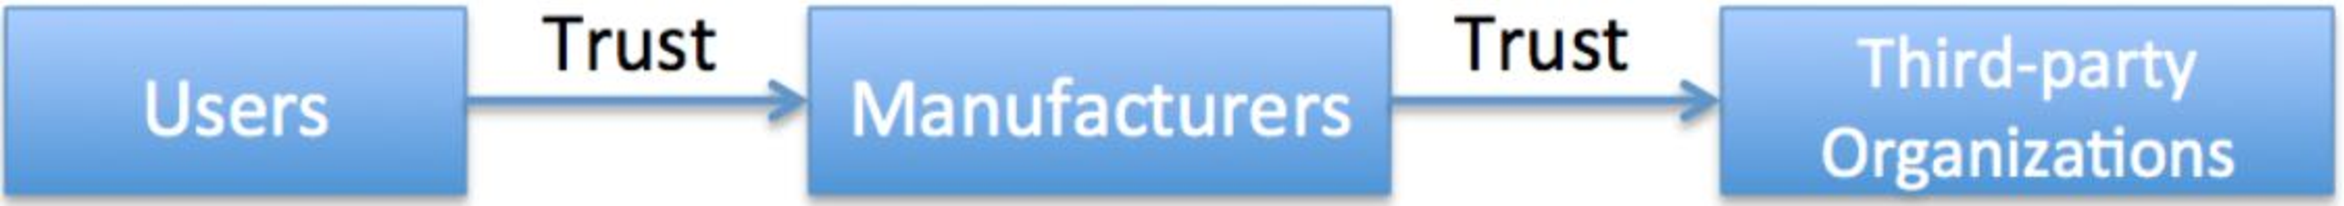
\includegraphics[width=0.75\columnwidth]{figures/trustchain.pdf}
	\caption{Trust Chain}
	\label{fig:trustchain}
\end{figure}

In all, based on the interview results, users are well aware of who is collecting, storing, and sharing their data. They have a demand of controlling the data flows to different Second-Parties or Third-Parties. The designers of future IoT privacy-setting interfaces should solve the challenges of differing various Second-parties and Third-Parties, and providing suitable access control options available to users of different IoT contexts.

\subsection{IoT Usability and Acceptability}
We now present the effect that usability of the IoT devices has on the acceptability to IoT systems/devices. We first describe the "convenience" and then discuss "control".

\subsubsection{Convenience and Usability}
From our study, we observed that one of the most important aspect of usability is convenience. Convenience in case of IoT can be treated as the ease with which the IoT systems/devices offers functionality. Convenience can simply be a feedback which is provided by the temperature sensors in an household IoT system or the various recommendations provided by a smart assistant (e.g. Amazon Echo) in a way that it eases the shopping experience on online shopping websites (e.g. Amazon.com). One of the users was asked about how they would feel being in an IoT environment replied by saying, ``Excited actually! When you describe that I don't know if that's sharing your same excitement but.. umm it actually is exciting to me because its so wonderfully convenient, so beautifully convenient." The same participant further went on saying ``I love it. I mean it would be awesome to look at my phone right now and say 'oh! My door's unlocked'. Actually my brother has that, actually he can check his phone can look if the door locks. And it's really cool! You don't have to worry when you go out on a trip. Or you can control the A/C if you forgot. It's really cool."  It is clear from this statement that convenience of use of IoT systems/devices is directly associated with the acceptability. Almost all of our participants pointed out the same thing in a similar way. The convenience offered through IoT systems/devices by enabling the users with a common platform from where they can easily connect with their devices goes a long way in improving the overall usability of the systems and thereby impacts the acceptability of IoT in its totality. 
%Usability for a few users also encompasses the aesthetics of any system which is evident from the statements made by participants.

\subsubsection{Being in Control and Usability}
From our study, we found that users are al well-aware of being in control when they are considering whether to adopt an IoT system. Another interesting aspect of control is that it is highly dependent on the information about the state of the system. Arguably, any individual will try to control something only when they are aware that it needs to be controlled or that it can be controlled. Therefore, being notified is primarily important before being able to control any aspect of the system. One of the participants when questioned about their opinion of overall usability of any device, mentioned enthusiastically that "I am excited by the idea that me being able to control what they want to do. I am less excited by the idea that them doing autonomously control what they want because some company told them to do it. Luckily the technology is so dumb right now. It's so linear, that it's not good at anticipating the things. But when it gets smarter, as long as it knew that I was an individual who would care, I think the same technology would allow you to totally automate your life but it would allow me to pick and choose which parts to automate". Even though users like a scenario of having everything automated, they still want to believe that they are in a position to control and are always aware of everything that the system is handling. It is evident from the comments that users want to keep absolute automation as a feature, but would probably completely rely on it when they have absolute confidence over its capability to handle things autonomously. A similar example in this regard would be the case of a pilot operating a commercial aircraft who would be prefer it more if the airplane were on autopilot while cruising. Although, he would also like to have the system informing him about the vital stats of the airplane while it's on autopilot. He would rather rely on his/her skills during landing and take-off of the aircraft. Lack of confidence in automated systems during decisive moments is a common trait found in human beings which in this case is clearly exhibited by the pilot~\cite{namara2018potential}.

\subsubsection{Being Notified and Being in Control}
``Control" can be the complete manual control of the system or it can be a situation where the user is notified regarding something which can be changed or altered subject to manual intervention. This is basically the system saying that it has an affordance which the user can utilize to better suit his/her convenience. In such a situation, the notification system (perhaps an application for IoT installed on the user's tablet) forms an interface between the machine and the user which serves as a medium to control the degree of automation. The entire idea behind having such an interface is to provide the user with control without compromising convenience. This phenomenon is depicted in the figure~\ref{fig:interface}.
\begin{figure}
	\centering
	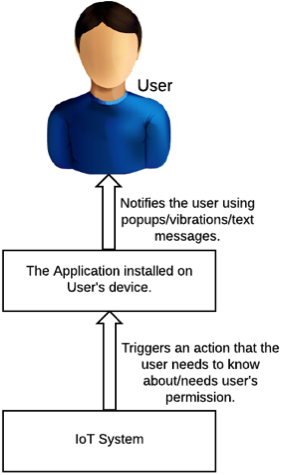
\includegraphics[width=4cm, height=6.3cm]{figures/interface.png}
	\caption{An interface for providing the user with "control"}
	\label{fig:interface}
\end{figure}

The assumption here is that the user is being notified about the several important aspects of the system. Being notified even after allowing something to take place is a requirement prevalent among many participants. One of the participants explicitly mentioned he would like periodic reminders about what is being recorded. This leads us to another interesting aspect of such a scenario which is the 'trust'. We assume that the user trusts the feedback from the system. The notification is perceived by the user as a kind of feedback and this leads to an impression of control in the user's mind where he/she is the master and the system is the apprentice. We think this situation is paramount in establishing trust and all participants desired it.

\section{Summary}
Based on the above analysis on our results, we see that when making the decision of whether to adopt the IoT technology, the users usually consider the trade-off between privacy and usability as against affordability (See Figure~\ref{fig:AcceptingProcess}). If the usability and privacy overweight the price, users will more likely to adopt an IoT system. In terms of the usability, if the users find the IoT systems can make their life easier, they will be more inclined to accept it. In terms of privacy, the users primarily make judgments based on the trust they have on the brand/manufacturer and its public image. For example, one of our participants mentioned that he would trust Apple when it comes to sharing of information, this participant had immense trust in Apple, based on some great reports recently published in newspapers. Hence, if they trust a brand with their data, they will have a better resolution of their privacy concerns, which would eventually lead to them accepting the technology. It is evident that the brand image will certainly play a key role in new users accepting the IoT technology.

Based on the insights gained from this study, we encourage the designers of IoT privacy-setting interfaces to face the difficult challenge of maximizing the usability and the privacy control of the user interface while minimizing the privacy threats to the users. However, since people differ extensively in their privacy settings~\cite{olson2005study}. At the same time, the vast number of different IoT devices makes choosing adequate privacy settings a very challenging task that is likely to result in information and choice overload~\cite{williams2016perfect}. Under these circumstances, a data-driven design approach seems promising since we could cluster similar users and summarize their privacy preference to generate a set of ``smart profiles" for new users to choose from in our IoT privacy-setting interface. We discuss this data-driven approach in the following chapters.
